\documentclass{article}


\usepackage{arxiv}

\usepackage[utf8]{inputenc} % allow utf-8 input
\usepackage[T1]{fontenc}    % use 8-bit T1 fonts
\usepackage{hyperref}       % hyperlinks
\usepackage{url}            % simple URL typesetting
\usepackage{booktabs}       % professional-quality tables
\usepackage{amsfonts}       % blackboard math symbols
\usepackage{nicefrac}       % compact symbols for 1/2, etc.
\usepackage{microtype}      % microtypography
\usepackage{lipsum}
\usepackage{graphicx}
\usepackage{outlines}
\usepackage{amsmath,amsthm,amssymb}
\usepackage{float}
\setlength{\parskip}{1em}
\setlength{\parindent}{0em} 
\newcommand{\N}{\mathbb{N}}
\newcommand{\Z}{\mathbb{Z}}
\newcommand{\Q}{\mathbb{Q}}
\newcommand{\R}{\mathbb{R}}
\newcommand{\C}{\mathbb{C}}
\newcommand{\F}{\mathbb{F}}
\newcommand{\V}{\mathcal{V}}
\newcommand{\U}{\mathcal{U}}
\newcommand{\W}{\mathcal{W}}
\newcommand{\K}{\mathbb{K}}
\newcommand{\PS}{\mathbb{S}}
\newcommand{\id}{\II}
\newcommand{\Pol}{\mathbb{P}}
\newcommand{\sls}{\mathcal{S}}
\newcommand{\vv}{{\bm{v}}}
\newcommand{\uu}{\bm{u}}
\newcommand{\cc}{\bm{c}}
\newcommand{\ww}{\bm{w}}
\newcommand{\ee}{\bm{e}}
\newcommand{\ff}{\bm{f}}
\newcommand{\hh}{\bm{h}}
\newcommand{\bfa}{\bm{a}}
\newcommand{\bfy}{\bm{y}}
\newcommand{\zz}{\bm{z}}
\newcommand{\pp}{\bm{p}}
\newcommand{\bfo}{\bm{0}} 
\newcommand\nulvec{\bm{0}}
\newcommand\nulmat{\bm{O}}
\newcommand\nulvecSet{\Set{\nulvec}}
\newcommand{\bfO}{\bm{O}}
\newcommand{\bfalp}{\bm{\alpha}}
\newcommand\la{\langle}
\newcommand\ra{\rangle}
\newcommand\E{\mathbb{E}}

\newcommand\Ein{E_{in}}
\newcommand\Eout{E_{out}}

\newenvironment{theorem}[2][Theorem]{\begin{trivlist}
\item[\hskip \labelsep {\bfseries #1}\hskip \labelsep {\bfseries #2.}]}{\end{trivlist}}
\newenvironment{lemma}[2][Lemma]{\begin{trivlist}
\item[\hskip \labelsep {\bfseries #1}\hskip \labelsep {\bfseries #2.}]}{\end{trivlist}}
\newenvironment{exercise}[2][Exercise]{\begin{trivlist}
\item[\hskip \labelsep {\bfseries #1}\hskip \labelsep {\bfseries #2.}]}{\end{trivlist}}
\newenvironment{problem}[2][Problem]{\begin{trivlist}
\item[\hskip \labelsep {\bfseries #1}\hskip \labelsep {\bfseries #2.}]}{\end{trivlist}}
\newenvironment{question}[2][Question]{\begin{trivlist}
\item[\hskip \labelsep {\bfseries #1}\hskip \labelsep {\bfseries #2.}]}{\end{trivlist}}
\newenvironment{corollary}[2][Corollary]{\begin{trivlist}
\item[\hskip \labelsep {\bfseries #1}\hskip \labelsep {\bfseries #2.}]}{\end{trivlist}}
\newcommand\arrows[3]{
        \begin{matrix}[c]
        \ifx\relax#1\relax\else \xrightarrow{#1}\fi\\
        \ifx\relax#2\relax\else \xrightarrow{#2}\fi\\
        \ifx\relax#3\relax\else \xrightarrow{#3}\fi
        \end{matrix}
}
\newcommand\inner[1]{\la#1\ra}
\newcommand\m[1]{\begin{pmatrix}#1\end{pmatrix}} 

\newcommand\vecnorm[1]{\lVert #1 \rVert}    
\newcommand{\lt}{\ensuremath <}
\newcommand{\gt}{\ensuremath >}


\graphicspath{ {./images/} }
\title{Lecture Notes on Neural Networks\\Machine Learning E20}


\author{
 Mathias Ravn Tversted \\
  Department of Computer Science\\
  Aarhus University\\
  Åbogade 34, 8200 Aarhus N \\
  \texttt{Tversted@post.au.dk} \\
  %% examples of more authors
  %% \AND
  %% Coauthor \\
  %% Affiliation \\
  %% Address \\
  %% \texttt{email} \\
  %% \And
  %% Coauthor \\
  %% Affiliation \\
  %% Address \\
  %% \texttt{email} \\
  %% \And
  %% Coauthor \\
  %% Affiliation \\
  %% Address \\
  %% \texttt{email} \\
}

\begin{document}
\maketitle
\tableofcontents
\newpage

\section{Introduction}
  Deep Learning uses neural networks to make simple and complex feature extraction from images and maps these features to different outputs. One of the most common uses is image classification, but there are a lot of different genres all from image generation to image transformation.

\section{Neural Network}
  A Neural Network is a connection of nodes that goes from some inputs and some biases to some outputs. These connections have different weights which is what we try to make better during training. To add more complexity and control each node can execute an activation function.
  
  Neural networks as functions have a lot of parameters and are quite abstract, but the idea is that by tweaking these many parameters and layers, that we have ``hone in on'' some target function.
  
  Neural networks are composed of many different types of functions.

\section{Fully connected networks}
    A fully connected layer is a layer in which there are multiple neurons. In such a layer, each neuron is connected to each neuron in the previous layer.
    
    This can make computation every effective, because this can be done with vector (grouped together to form matrices) operations, which can be GPU accelerated.

  Our calculations are then as follows:
  Let $\phi$ be the activation function for the layer (explained in a bit). $x$ is the input, $W$ are the weights for the connections between two layers, and $b$ are the biases for for that layer.
  \begin{align}
    \phi^k(\phi^{k-1}(\dots\phi^2(\phi^1(xW^1+b^1)W^2+b^2)\dots)W^k+b^k)
  \end{align}
\section{Activation functions}
  In each layer, we can have a function, called an activation function, which takes the inputs to each neuron and outputs the output of the function to the next layer.
  
  Common ones are:
  \begin{itemize}
    \item Identity function. 
    \item ReLU (Rectified Linear Unit): $f(x) = max(0, x)$ 
    \item Sigmoid: $\sigma(z) = \frac{1}{1+e^{-z}}$
    \item Softmax: $\softmax(z)_i = \frac{e^{z_i}}{\sum_{j=1}^{n}{e^{z_j}}}$
  \end{itemize}
  These can have many useful properties.
  
  ReLU is useful in that it allows neurons to be "turned off" if they do not receive sufficient output. This is useful, as it allows for flexibility in training, and for certain neurons to do certain things, rather than always having to contribute to the output. 
  
  Sigmoid squishes outputs into the interval $[0, 1]$, but has vanishing gradients problem.
  
  Softmax is often used in the last layer for multinomial logistic regression. This is when we want to predict the class of an input with several predictions.
  
  
\section{Convolutions}
  Convolutions act as a kind of ``filter'' on images that can be \emph{trained} to identify (more abstract) features. A $k \times k$ convolution is specified by a $k \times k \times c$ tensor, where $k$ is often odd, so it can center on a pixel. The idea is to ``slide'' it across the image with some stride $s$. (Tells us how much we shift). 
  
  An entry in the output tensor is then a linear combination of the entries in the corresponding convolution window as well as the weights of the convolution. The weights are shared. 

  \textbf{Example: Edge detection}: 
  \begin{equation}
    E = \begin{bmatrix}
      -1 & -1 & -1 \\
      -1 & 8 & -1 \\
      -1 & -1 & -1
    \end{bmatrix}
  \end{equation}
  Which checks if the middle pixel is different from average. This is \emph{translation invariant} as it finds the same pattern. This is important, because these kinds of convolutions allow us to find the same things in different images. 

  Convolutions reduce the size of images, but with $\frac{k-1}{2}$ $0$s as padding, it can center on every pixel and produce the same output size. 

  \emph{Scale-invariance} however, could be a problem. 

    \subsection{Pooling}
      Is a $k \times k$ function of $k$ elements $\phi : R^k \rightarrow R$ with stride $s$. For example, max-pooling where the output is the maximum value in the window. There is also mean and min. Pooling with stride $s > 1$ reduces image size by factor $s$. 
  
\section{Training neural networks}
  Training neural networks is usually done with techniques such as \emph{(stochastic/mini-batch) gradient descent}, with any point-wise loss function $E_{in}(w) = \frac{1}{n}\sum_{i=1}^{n}{L(h(x_i), y_i)}$
  
  \textbf{Mini-batch SGD}:
  \begin{itemize}
    \item Initialise $w$ (e. g random $N(0,1)$)
    \item While more time (epochs may be fixed):
    \item \begin{enumerate}
      \item Shuffle $(x_1, y_1), \cdots, (x_n, y_n)$
      \item For $i = 1, \cdots, n/B$:
      \item Let $(x_1', y_1'), \cdots, (x_n', y_n')$ be the next batch
      \item $g = \frac{1}{B} \sum_{i=1}^{B}{\nabla L (w(x_i'), y_i')}$
      \item $w = w - \eta g$
    \end{enumerate}
  \end{itemize}

\section{Forward/Backward Pass}
  When we evaluate a Neural Network we call it a Forward Pass. That simply follows the activation rules given in each node and passes the values added together forward.\\
  These Forward Passes are differentiable so we can calculate which way we should move the different weights in order to get better results. This process is called a Backward Pass.\\
  
  An example is a simple neural network from TA Class: $nn(x) = w x$.\\
  We wish to optimize this using least squares error: $e = (y-nn(x))^2$\\
  \begin{figure}[H]
      \centering
      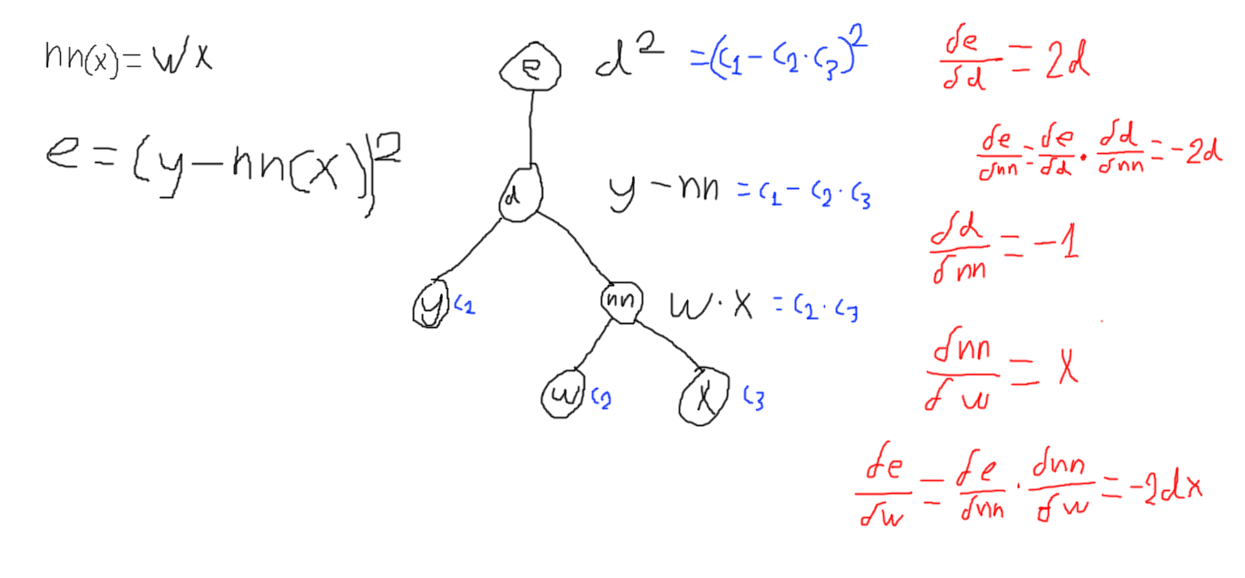
\includegraphics[width=0.8\textwidth]{ForwardNBaclPass.png}
      \caption{Example of Forward and backward pass}
      \label{fig:my_label}
  \end{figure}


\section{Overfitting}
  With enough states a neural network can learn to produce all the desired outcomes, but might not generalize that well to new data.
  There are multiple methods that can help mitigate this overfitting of the training data.
  \subsection{Validation - Early Stopping}
    You can use a validation set to test the model while training it. Then when you see a increase in the validation that means that the model is beginning to overfit.
    You can stop there or in practice check for a multiple epochs and if it keeps increasing then stop and use the model that had the best validaiton error.
    Normally the validation set is about 20\% of the test set.
  \subsection{Regularization - Weight Decay}
    Sometimes the weights tend to skyrocket to fit the training set better. 
    We can fix this by punishing big weights as a part of the in-sample error function.\\
    $E_{in}(nn) = \frac{1}{n}\sum_{i=1}^n L(nn(x_i), i) + \lambda \sum_{w\in nn}w^2$.
    We use the variable $\lambda$ to specify how much it should punish big weights. A good value is around $0.01$ we found from tests in the second handin.
  \subsection{Dropout - Not pensum}
    We can modify our Neural Network so it has some chance of not using the value from a node. This is called dropout and is very effective, but not very technical to implement.

\section{Cross-entropy loss}

    Recall that for multinomial regression, we use softmax as our loss function 
    \begin{align}
      L(h(x), y) = -ln(y^T softmax(x^TW))
    \end{align}
    With $K$ entries summing to $1$. For multiclass classification however, this can be problematic, as the target will contain $1$ in several entries. 

    If we want to do multi-class classification, we can use cross-entropy loss as our loss function. This can be considered a generalisation of softmax for multinomial regression. 

    Entropy is defined as $-H(S) = \sum_{i=1}^{k}{p_i log_2(p_i)}$, but if we substitute $log_2(p_i)$ for our hypothesis $h(x)$, we will gain higher values as our hypothesis diverges from the actual probabilities. Cross entropy loss is then defined as $-L(h(x), y) = \sum_{j=1}^K y_{i}ln(h(x_i)_j)$

    The In-sample Error is defined using Cross-entropy loss for $K$-label neural networks as follows:\\
    $E_{in}(h) = -\frac{1}{n}\sum_{i=1}^n\sum_{j=1}^K y_{i,j}ln(h(x_i)_j)$

    It also means that we can remove softmax layers and include it in the loss function instead. 

\end{document}
